\chapter{Dinámica semiclásica del electrón en la red de Tight Binding en campos rápidamente oscilantes}

\section{Método de Kapitza en la dinámica clásica de una partícula en presencia de un campo externo rápidamente oscilante}\label{cap:6}

Se quiere estudiar el procedimiento de Kapitza para modelar partículas clásicas en presencia de fuerzas externas rápidamente oscilantes. El siguiente procedimiento sigue los presentados por Kapitza \cite{kapitza} y Landau \cite{landau},  para modelar la dinámica de partículas clásicas sometidas a campos rápidamente oscilantes.

La ecuación de movimiento de una partícula de masa $m$, que experimenta un potencial $U$ independiente del tiempo y una perturbación $f(x,t)$ rápida, está dada por la segunda ley de Newton: 

\begin{equation}\label{eq:6.1}
    m\ddot{x}=-\frac{\partial U(x)}{\partial x}+f(x,t)
\end{equation}

Se describe una fuerza externa que incluye todos los posibles armónicos de $\omega$ modulados por una función $f_n(x)$. Por simplicidad, se supone que $f_n(x)=f_{-n}(x)$ y se escribe como serie de Fourier, tal como se muestra a continuación:

\begin{equation}\label{eq:6.2}
    f(x, t) = \sum^{\infty}_{n=-\infty} f_n(x)e^{in\omega t},
\end{equation}

Donde $f_n(x)$ y $\omega$ son grandes comparados con las amplitudes y frecuencias naturales del movimiento lento. Por la naturaleza de las fuerzas, que actúan sobre la partícula, se puede deducir que la partícula efectúa un movimiento rápido debido a la fuerza oscilante; y al mismo tiempo, presenta un movimiento suave debido a la fuerza $U(x)$ de oscilación lenta.
Se puede separar el movimiento de la partícula en un movimiento rápido y otro lento. Esta situación se expresa matemáticamente con la expresión:

\begin{equation}\label{eq:6.3}
    x(t) = X(t) + \xi(t),
\end{equation}

Donde $\xi$ representa el movimiento rápido y se supone pequeño y de promedio cero en un periodo de movimiento rápido  ($T=2\pi/\omega$). Se supone, también, que en períodos de tiempo pequeños  los cambios de $X(t)$ son insignificantes. 

Sustituyendo la ecuación \ref{eq:6.3} en \ref{eq:6.1}, y expandiendo el lado derecho de la ecuación \ref{eq:6.1} en serie de Taylor alrededor de $\xi=0$ a primer orden, se tiene la ecuación:

\begin{equation}\label{eq:6.4}
    m(\ddot{X}(t) + \ddot{\xi}(t))=-\frac{\partial U(X)}{\partial X}-\xi\frac{\partial^2 U(X)}{\partial X^2}+f(X,t)+\xi\frac{\partial f(X,t)}{\partial X}
\end{equation}

Las derivadas en el tiempo que aparecen en \ref{eq:6.4} son funciones suaves, en el sentido que no varían mucho para tiempos del orden del periodo pequeño. Se puede separar entonces los movimientos rápido y lento de la siguiente manera:

\begin{equation}\label{eq:6.5}
    m\ddot{X}(t) =-\frac{\partial U(X)}{\partial X}-\xi\frac{\partial^2 U(X)}{\partial X^2}+\xi\frac{\partial f(X,t)}{\partial X}
\end{equation}

\begin{equation}\label{eq:6.6}
    m\ddot{\xi}(t)=f(X,t)
\end{equation}

Se integra, la ecuación \ref{eq:6.6} en la variable temporal y se obtiene una expresión  para $\xi$ (suponiendo condiciones iniciales apropiadas que anulan el término secular):

\begin{equation}\label{eq:6.7}
    \xi=-\frac{1}{m\omega^2}\sum^{\infty}_{n=-\infty} \frac{f_n(X)e^{in\omega t}}{n^2}
\end{equation}
 
Conociendo una expresión para $\xi$, se puede ahora calcular el valor promedio de $\ddot{x}(t)$ en un periodo rápido, teniendo en cuenta que $\overline{\ddot{\xi}(t)}=0$:

\begin{equation}\label{eq:6.8}
    m\overline{\ddot{X}}(t) =-\overline{\frac{\partial U(X)}{\partial X}}-\overline{\xi\frac{\partial^2 U(X)}{\partial X^2}}+\overline{\xi\frac{\partial f(X,t)}{\partial X}}
\end{equation}

Recordando que $U(X)$ se considera constante para periodos pequeños y que $\xi$ tiene promedio nulo en ese mismo periodo. Además, se puede calcular $\overline{\xi\frac{\partial f(X,t)}{\partial X}}$ y obtener la siguiente ecuación:

\begin{equation}\label{eq:6.9}
     m\overline{\ddot{X}}(t) =-\frac{\partial U}{\partial X}-\frac{1}{2m\omega^2}\frac{\partial}{\partial X}\sum_n \frac{f_n^2(X)}{n^2}
\end{equation}

Se puede definir el potencial efectivo de una partícula sometida a fuerzas rápidamente oscilantes como se presenta en el resultado \ref{eq:6.11}:

\begin{equation}\label{eq:6.10}
    m\overline{\ddot{X}}=-\frac{\partial U_{eff}(X)}{\partial X}
\end{equation}

\begin{equation}\label{eq:6.11}
U_{eff}(X)=U(X)+\frac{1}{2m\omega^2}\sum_n \frac{f_n^2(x)}{n^2}   
\end{equation}

Se observa que el potencial experimenta una corrección que es inversamente proporcional a la masa y al cuadrado de la frecuencia de la fuerza rápidamente oscilante. Además es directamente proporcional a la suma del modulo cuadrado de los armónicos de la fuerza y que la corrección tiene una dependencia en $X$. En el límites $\omega \rightarrow \infty$ el término de corrección del potencial se hace insignificante y el efecto de la fuerza externa sobre la dinámica de la partícula será nulo.

%%%%%%%%%%%%%%%%%%%%%%%%%%%%%%%%%%%%%%%%%%%%%%%%%%%%
\section{Dinámica semiclásica del electrón en la red de enlace fuerte en presencia de campos externos}\label{cap:7}

%En este capitulo se estudia el modelo semiclásico para la dinámica del electrón en la red. Este modelo permite predecir de forma sencilla el comportamiento del electrón en la red en presencia de campos externos, sin embargo existen ciertas condiciones que limitan la aplicación de este modelo, las cuales son aclaradas. Se presenta el concepto de masa efectiva del electrón y la deducción de su expresión matemática a partir de las ecuaciones de movimiento semiclásicas. Se presenta además la aplicación del modelo semiclásico para el caso del electrón en la red en presencia de un potencial perturbativo lineal, cuyo resultado son las oscilaciones de Bloch. Este capítulo abre el camino para el estudio semiclásico que se presenta mas adelante sobre el electrón en la red en presencia de campos rápidamente oscilantes (capítulo \ref{cap:9}). 

El modelo semiclásico describe la respuesta de los electrones en la red a un campo externo aplicado. Para que este modelo sea válido, las variaciones del campo en el espacio deben ser muy pequeñas comparadas con las dimensiones del paquete de onda del electrón. Estos campos dan origen a fuerzas clásicas que describen el movimiento del paquete de onda. La segunda condición en el modelo semiclásico es que la periodicidad de la red debe ser pequeña comparada con las dimensiones del paquete de onda del electrón. En esta situación, el potencial de la red no puede tratarse clásicamente (ver figura \ref{fig:7.1}). Por lo tanto, el modelo semiclásico trata las fuerzas externas clásicamente, mientras que el potencial cristalino es tratado cuánticamente \cite{ashc}.

\begin{figure}[H]
    \centering
    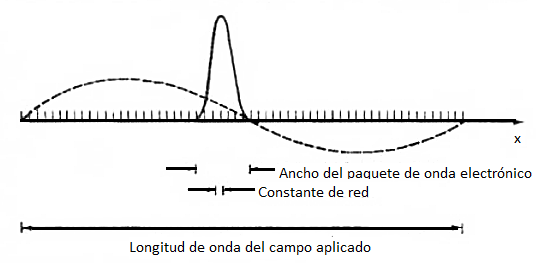
\includegraphics[scale=.9]{imagenes/dinamica-semiclasica.png}
    \caption{Electrón en una red periódica en presencia de un potencial periódico externo, Modificado de Ashcroft y Mermin \cite{ashc} }
    \label{fig:7.1}
\end{figure}

El modelo semiclásico, describe (en ausencia de colisiones) la velocidad $\dot{x}$ y la fuerza $\hbar k$, que experimenta el paquete de onda del electrón en presencia de un campo externo; esta predicción es posible en conocimiento de la relación de dispersión $\mathcal{E}_n(k)$. Dada la función $\mathcal{E}_n(k)$ el modelo semiclásico permite calcular la posición $x$ y el vector de onda $k$ asociado a éste para una banda $n$. En presencia de campos eléctricos $E(x,t)$ y magnéticos $\mathcal{H}(x,t)$ la posición y el vector de onda pueden ser calculados siempre y cuando la posibilidad de intercambio de banda $n$ sea descartada. Entonces las ecuaciones de movimiento del electrón serán las siguientes:

\begin{equation}\label{eq:7.1}
    \dot{\textbf{x}}=\textbf{v}_n(k)=\frac{1}{\hbar}\frac{\partial \mathcal{E}_n(k)}{\partial k}
\end{equation}

\begin{equation}\label{eq:7.2}
    \hbar\dot{\textbf{k}}=-e\left[\textbf{E}(x,t)+\frac{1}{c}\textbf{v}_n(k)\times \mathcal{H}(x,t)\right]
\end{equation}

En el modelo semiclásico, no puede haber dos electrones cuyos valores de $k$ difieran por una constante de red reciproca $K$, puesto que las funciones que describen al electrón son periódicas, de periodo $K$, y en consecuencia se estaría hablando del mismo electrón \cite{ashc}.

El método de Kapitza, usando el enfoque semiclásico permite crear un nuevo modelo que describe la dinámica del electrón en la red en presencia de campos rápidamente oscilantes. Mas adelante se encontrará que es posible obtener una fórmula general del potencial efectivo para el electrón en presencia de cualquier potencial que cumpla con las condiciones semiclásicas que se han estudiado en esta sección (capítulo \ref{cap:9}).

\subsection{Masa efectiva}

Se puede describir la manera como un electrón responde a fuerzas externas definiendo una nueva cantidad llamada masa efectiva del electrón:

\begin{equation}\label{eq:7.3}
    \frac{1}{m^*}=\frac{1}{\hbar^2}\frac{\partial^2 \mathcal{E}(k)}{\partial k^2}
\end{equation}

Esta ecuación se obtiene de las ecuaciones del movimiento semicásico del electrón
e implica que es posible para el electrón tener masa efectiva positiva o negativa. La masa efectiva es positiva cuando la relación de dispersión tenga una curvatura hacia arriba y negativa cuando la curvatura sea hacia abajo, incluso puede haber masa cero en los puntos de inflexión de la curva.

Para un electrón libre la relación de dispersión tiene la expresión cuadrática:

\begin{equation}\label{eq:7.4}
    \mathcal{E}(k)=\frac{\hbar^2k^2}{2m}
\end{equation}

Entonces la masa efectiva, como es de esperarse, es la misma que la masa regular del electrón:

\begin{equation}\label{eq:7.5}
    m^*=m
\end{equation}

Para un electrón en la red de \textit{Tight Binding} la relación de dispersión tiene una forma totalmente diferente a la del electrón libre:

\begin{equation}\label{eq:7.6}
    \mathcal{E}(k)=\mathcal{E}_0-2A\cos(ka)
\end{equation}

En consecuencia la masa efectiva del electrón en la red de \textit{Enlace Fuerte}, tomando $\hbar$=1, resulta ser:

\begin{equation}\label{eq:7.7}
    m^*=(2Aa^2\cos(ka))^{-1}
\end{equation}

A continuación se presenta un gráfico referencial de la masa efectiva del electrón en la red de enlace fuerte como función de $k$, se ha dibujado también la curva de la relación de dispersión para que se pueda apreciar la relación entre ambas.

\begin{figure}[H]
    \centering
    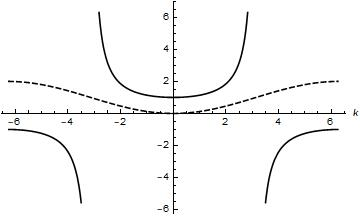
\includegraphics{imagenes/masa-efectiva.jpg}
    \caption{Linea solida: Masa efectiva, Linea discontinua: Relación de dispersión}
    \label{fig:my_label}
\end{figure}

En la figura se puede observar que el cambio de concavidad en la curva de relación de dispersión provoca un cambio de signo en la masa efectiva del electrón en la red de \textit{Tight Binding}. Este cambio de signo también se puede interpretar como un cambio de signo en la carga del electrón, pasando de ser atraído por el pozo de potencial a ser repelido por este en la zona de masa efectiva negativa.

\subsection{Oscilaciones de Bloch}\label{cap:7.2}

En 1928, Bloch demostró teóricamente que un paquete de ondas electrónicas, compuesto por una superposición de estados de una sola banda, bajo la acción un campo eléctrico externo aplicado alcanza su punto máximo en un determinado cuasi momentum $k$ y presenta oscilaciones periódicas en el momento y el espacio real, si se descartan las transiciones entre bandas \cite{Shah}.

La dinámica de los electrones de Bloch en un campo eléctrico homogéneo es un problema de larga data en el estudio en la \textit{Física del Estado Sólido}, si se considera un electrón sin colisión en una red periódica en una dimensión, con un movimiento normal a los planos de la superred. La ecuación de movimiento del electrón en presencia de un campo eléctrico uniforme $E$, paralelo a k, se escribe según las ecuaciones siguientes: 

\begin{equation}\label{eq:7.8}
    \frac{\hbar dk}{dt} = -eE
\end{equation}

\begin{equation}\label{eq:7.9}
    k(t)=k_0-\frac{eEt}{\hbar} 
\end{equation}

El electrón, se mueve hasta alcanzar el punto máximo de la banda, entonces es reflejado por ésta en la frontera de la \textit{Zona de Brillouin} (\textit{Reflexión de Bragg}) e invierte su movimiento. En el caso ideal, se puede ignorar por completo la dispersión causada por los iones de la red o imperfecciones y el electrón efectúa \textit{Oscilaciones de Bloch} de periodo dado por la ecuación \ref{eq:7.9}, donde $a$ es la constante de la red y $h$ la constante de Planck.

\begin{equation}\label{eq:7.10}
    \tau_B=\frac{\hbar}{eEa}
\end{equation}

Se considera el movimiento del electrón en el espacio real con la relación de dispersión en el \textit{Enlace Fuerte} y la expresión para la velocidad del electrón en el modelo semiclásico \cite{kittel}:

\begin{equation}\label{eq:7.11}
\mathcal{E}(k)=\mathcal{E}_o-2A\cos(ka)   
\end{equation}

\begin{equation}\label{eq:7.12}
v=\frac{1}{\hbar}\frac{d\mathcal{E}}{dk}
\end{equation}

Sustituyendo el resultado \ref{eq:7.11} en \ref{eq:7.12} se puede obtener la posición del electrón en función del tiempo, que resulta ser una función periódica con período de oscilación $\tau_B$:

\begin{equation}\label{eq:7.13}
    x=-\frac{2A}{Ee}\cos(\frac{aeE}{\hbar}t)
\end{equation}

 Este resultado confirma la existencia teórica de las oscilaciones de Bloch cuya frecuencia en el espacio real es $\omega_B=\hbar/aeE$, y período igual a $\tau_B$. Se encuentra entonces que la respuesta del electrón en la red a un potencial lineal externo es totalmente diferente que en el espacio libre, para el cual la aceleración producida por un campo eléctrico homogéneo es constante \cite{kittel}. En este caso, el electrón experimenta oscilaciones alrededor de un punto de equilibrio.
 
En la ecuación \ref{eq:7.3} se observa que cuanto mayor sea la magnitud del campo eléctrico externo, la amplitud de las oscilaciones y el periodo de Bloch son menores. Por lo tanto la probabilidad de que el electrón sufra algún tipo de dispersión antes de terminar una oscilación de Bloch es menor. Las oscilaciones de Bloch son difíciles de observar experimentalmente en un sólido cristalino, debido a que la dispersión por impurezas o fonones impide la finalización de un solo período de oscilación \cite{raizen}. Esto hizo que la investigación en el campo de la dinámica oscilatoria de electrones en los sólidos haya tenido durante muchos años un interés sobre todo teórico. La obtención en los últimos años de materiales con constante de red $a$ de ordenes diez veces mayor a las convencionales y menor presencia de impurezas ha aumentado el atractivo de esta área de la Física del Estado Sólido \cite{wannier2}. Una de las condiciones para la observación de las oscilaciones de Bloch, es que el período de oscilación $\tau_B$ debe ser menor que el tiempo medio de viaje $\tau_m$, de lo contrario, el electrón experimentará una dispersión antes de poder observar alguna oscilación.


Para este proyecto de grado se ha querido considerar campos externos inhomogéneos y rápidamente oscilantes, con la finalidad de estudiar la dinámica del electrón en presencia de estos campos y observar posibles fenómenos oscilatorios y de localización del paquete de onda del electrón.
